\chapter{Technology Stack}

La scelta della tecnologia da impiegare è un aspetto fondamentale di ogni progetto, e questo chiaramente non fa eccezione. \\

Molti testi --- fra cui uno dei preferiti dall'autore\footnote{Si tratta di \cite{pragmatic}, un libro estremamente interessante, oltre che essenziale come spunto di riflessione per lo sviluppo personale e professionale di ogni informatico che osi definirsi programmatore.} --- hanno proposto analogie fra gli utensili di un artigiano e gli strumenti software di un qualaunque utlizzatore informatico. Sull'onda di questa metafora, una lima non adatta al tipo di materiale che si intende lavorare non potrà mai garantire risultati eccellenti, indipendentemente dalla bravuta dell'artigiano stesso. \\

Appare chiaro che una scelta sbagliata di tecnologie da utilizzare può condizionare negativamente l'esito di un qualaunque lavoro, pertanto occorre prestare particolare attenzione nel decidere quale tecnologia impiegare per raggiungere lo scopo.

\section{Strumenti Necessari}

    Messi da parte i vaneggiamenti poetici, all'atto pratico è evidente che gli strumenti di cui l'analisi ha bisogno sono in realtà pochi e piuttosto comuni:

    \begin{itemize}
        \item abbiamo a che fare con una certa quantità di dati $\rightarrow$ servirà un \textit{Data Base Management System}.
        \item occorre avere una comprensione generale dei dati $\rightarrow$ occorrerà un software che permetta di usare \textit{tecniche di visualizzazione}.
        \item dobbiamo lanciare degli algoritmi di \textit{data mining} $\rightarrow$ abbiamo bisogno di un software che li implementi.
    \end{itemize}

    Tutto questo è facilmente ottenibile impiegando gli strumenti che saranno descritti nelle prossime sezioni.

\section{Data Base Management System: MongoDB}

    \begin{figure}
        \centering
        \caption{logo del DBMS MongoDB}
        \label{mongodb_logo}
    	
\includegraphics[scale=0.70]{img/mongodb.png}
    \end{figure}

    La scelta del Data Base Management System è stata quella che ha impattato più di tutte il tipo di lavoro che è stato necessario fare.

    \subsection{La scelta di MongoDB}
    
        Sono state valutati principalmente due \textit{DBMS} candidati, entrambi \textit{open source}:

        \begin{itemize}
            \item \textbf{MySQL}, un \textit{DBMS} relazionale, rodato e ormai \textit{staple} nella manipolazione dati
            \item \textbf{MongoDB}, un \textit{DBMS} di nuova generazione che adotta invece il paradigma \textit{NoSQL} 
        \end{itemize}

        I dati che si hanno a disposizione sono in forma ovviamente relazionale --- cioè, sono tabelle. Utilizzare \textit{MySQL} potrebbe sembrare quindi una scelta tanto solida quanto ovvia, ma sul piano prestazionale il \textit{modello a documenti} di \textit{MongoDB} risulta sensibilmente più efficiente nel manipolare grandi quantità di dati molto diversi fra loro. \\

        La decisione che è stata infine presa --- \textit{utilizzare MongoDB} --- ha tenuto conto anche del valore didattico che ha l'imparare un nuovo paradigma di memorizzazione dati che trascende il classico modello relazionale.

    \subsection{Caratteristiche di MongoDB}

        Come si può banalmente leggere in \cite{mongowiki}: \\
        
        "\textbf{MongoDB} \textit{(da "humongous", enorme)} è un DBMS non relazionale, orientato ai documenti. Classificato come un database di tipo \textbf{NoSQL}, MongoDB si allontana dalla struttura tradizionale basata su tabelle dei database relazionali in favore di \textbf{documenti in stile JSON} con schema dinamico (MongoDB chiama il formato BSON), rendendo l'integrazione di dati di alcuni tipi di applicazioni più facile e veloce." \\

        La società MongoDB Inc mette a disposizione liberamente e gratuitamente una buona documentazione in \cite{mongodb}, la quale contiene tutte le informazioni necessarie per utilizzare almeglio il DBMS da loro sviluppato. 

        Oltre alla sua \textit{shell}, MongoDB espone delle \textit{API} per i principali linguaggi di programmazione. Questo aspetto è tornato molto utile per specificare le operazioni di \textit{preprocessing} in un linguaggio familiare e più facilmente gestibile del dialetto di Javascript nativo di MongoDB.

\section{Interazione col DBMS: Python}

    \begin{figure}
        \centering
        \caption{logo del linguaggio di programmazione Python}
        \label{python_logo}
    	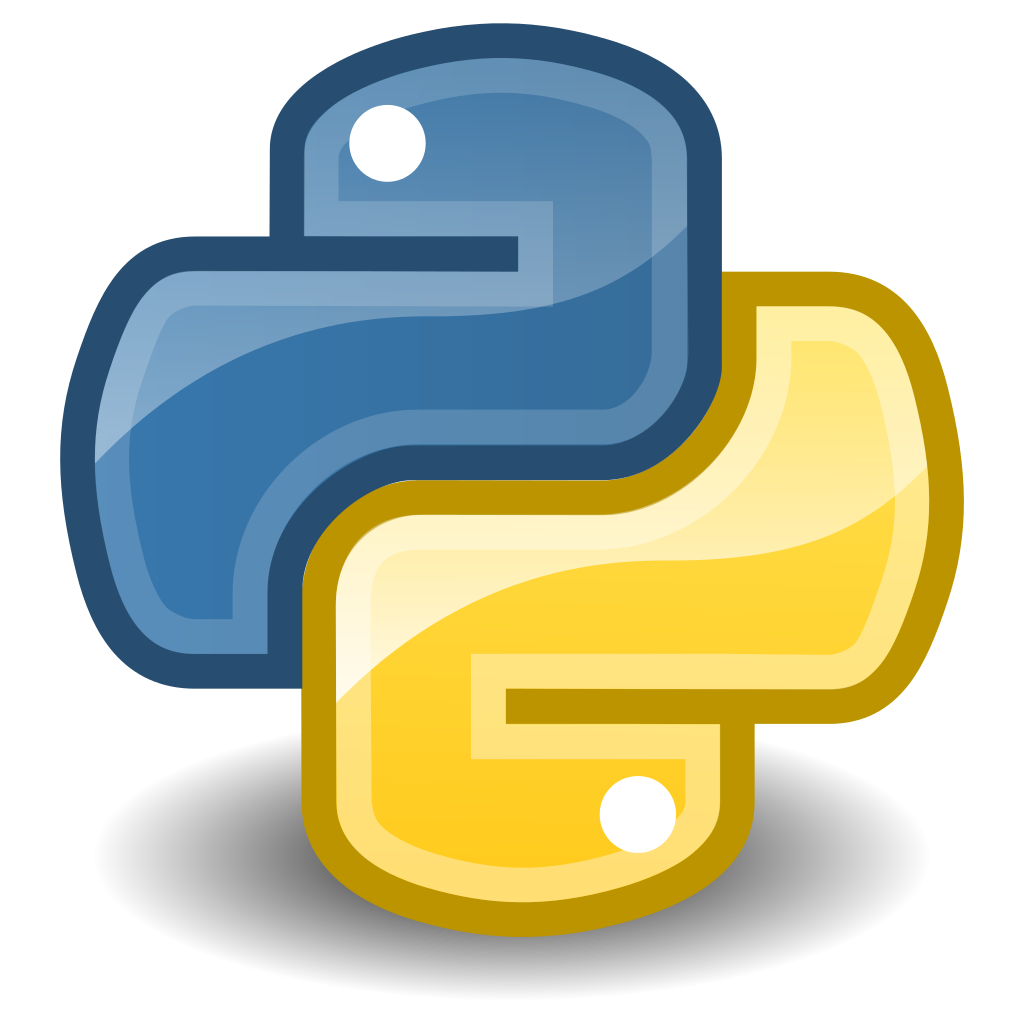
\includegraphics[scale=0.1]{img/python.png}
    \end{figure}

    A proposito di quando detto alla fine della sezione precedente, il linguaggio scelto è stato \textbf{Python}. Come si può leggere direttamente da \cite{pywiki}:\\

    "\textit{Python} è un linguaggio multi-paradigma, che ha tra i principali obiettivi \textit{dinamicità}, \textit{semplicità} e \textit{flessibilità}. Supporta il paradigma object oriented, la programmazione strutturata e molte caratteristiche di programmazione funzionale e riflessione." \\

    Il linguaggio Python ha una estesa e approfondita documentazione, messa a disposizione direttamente dalla Python Software Foundation in \cite{python}.

    \subsection{API per MongoDB: pymongo}

        \begin{figure}
            \centering
            \caption{schema riassuntivo del modello di lavoro con \textbf{pymongo}}
            \label{pymongo_logo}
    	    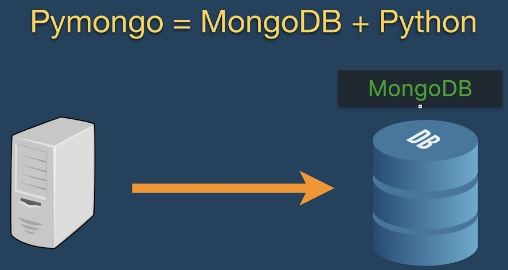
\includegraphics[scale=0.75]{img/pymongo.png}
        \end{figure}

        Una sintetica ma tremendamente efficace descrizione di che cosa è \textbf{pymongo} si può trovare direttamente nella sua documentazione, in \cite{pymongo}:\\

        "PyMongo is a Python distribution containing tools for working with MongoDB, and is the recommended way to work with MongoDB from Python." \\

        Ovvero: \\

        "PyMongo è una distribuzione di Python che contiene degli strumenti per lavorare con MongoDB, ed è la maniera raccomandata per avere a che fare con MongoDB da Python." \\







